\chapter{TikZ 绘图初步}

PGF ("portable graphics format") is the basic layer, providing a set of basic commands for producing graphics, and TikZ ("TikZ ist kein Zeichenprogramm" (German) or "TikZ is not a Drawing program") is the frontend layer with a special syntax, making the use of PGF easier. TikZ commands are prevalently similar to Metafont, the option mechanism is similar to PsTricks syntax. 
本章内容主要参考:\cite{WIKIBOOKS}.

\section{基本使用}

TikZ 可以直接在 .tex 文件中使用,也可以使用 TikZ 生产独立的图像文件,其模版如下:

\begin{minted}{latex}
\documentclass{standalone}
\usepackage{tikz}
\usetikzlibrary{<list of libraries separated by commas>}

\begin{document}

\begin{tikzpicture}[<options>]
<tikz commands>
\end{tikzpicture}

\end{document}
\end{minted}

\begin{remark*}
  每条绘图命令必须以分号结束。
\end{remark*}

先看一个简单的例子:

\inputminted{latex}{examples/tikz/preliminaries/standalone-example.tex}

生成的图像文件:

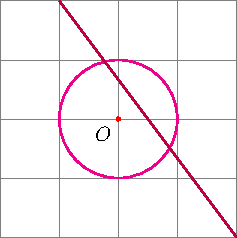
\includegraphics{examples/tikz/preliminaries/standalone-example.pdf}

\subsection{行内模式:\protect\verbum*{tikz} 命令}

\mint{latex}|\tikz[<options>]{<tikz commands>}|

One special option for this case is \mintinline{latex}{baseline = <dimension>}. Without that option the lower end of the picture is put on the baseline of the surrounding text. Using this option, you can specify that the picture should be raised or lowered such that the height \verbum{<dimension>} is on the baseline.

下面的代码演示了行内 TikZ 绘图效果:

\begin{texcode}
我们可以直接在行内绘制图形,如:直线\tikz \draw (0,0) -- (2em,1em);(注意
命令之后必须要以分号结束)。当不指定 baseline 参数时,图形的下端将与文本下端平齐,
当指定 baseline 参数时,图形的原点将定位到指定的高度,如:
\tikz{
  \draw (0,0) circle (1em); 
  \draw (0,0) rectangle (1em,1em);
}
\tikz[baseline=2em]{
  \draw (0,0) circle (1em); 
  \draw (0,0) rectangle (1em,1em);
}
\tikz[baseline=-3em]{
  \draw (0,0) circle (1em); 
  \draw (0,0) rectangle (1em,1em);
}
\end{texcode}

\subsection{\protect\verbum{tikzpicture} 环境}

\begin{minted}{latex}
\begin{tikzpicture}[<options>]
  <tikz commands>
\end{tikzpicture}
\end{minted}

例如绘制坐标轴:

\begin{texcode}
\begin{tikzpicture}[scale=.75]
  \draw[help lines] (-2,-2) grid (2,2);
  \draw[-latex] (-3,0) -- (3,0) node[below right] {$x$};
  \draw[-latex] (0,-3) -- (0,3) node[above left] {$y$};
  \node[below left] at (0,0) {$O$};
\end{tikzpicture}
\end{texcode}

\section{坐标}